\tikzset{
pics/dsig/.style n args = {2}{
	code = {
	\node at (#1,1) {#2};
	\draw (0,0) -- (1,0) -- (1,1) -- (2,1) -- (2,0) -- (3,0) -- (3,1) -- (4,1);
	}
	}
}

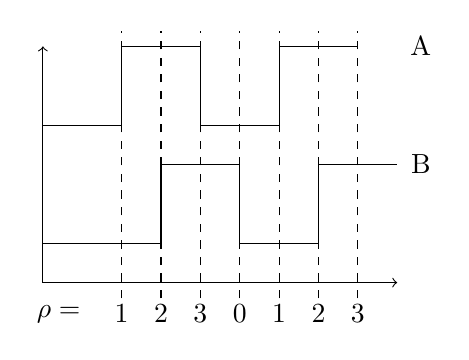
\begin{tikzpicture}[scale=1]
\node at (0.2,-.4) {$\rho=$};
\foreach \x/\n in {1/1,1.5/2,2/3,2.5/0,3/1,3.5/2,4/3}
{
	\draw[dashed] (\x,-.2) -- (\x,3.2);
	\node at (\x,-.4) {\n};
}

\draw[<->] (0,3) -- (0,0) -- (4.5,0);

% a signal
\draw pic[shift={(0,2)}] {dsig={4.8}{A}};

% b signal
\draw (0,.5) -- (.5,.5) pic {dsig={4.3}{B}};
\end{tikzpicture}
